\documentclass[fleqn,a4paper,12pt]{article}

%used Packages
\usepackage{standalone}		% Zum Einlesen aus anderen .tex-Files
\usepackage{geometry}		% Zur Bearbeitung des Layouts (Ränder,...)
\usepackage[german]{babel}
\usepackage[utf8]{inputenc}
\usepackage{amsmath}		% Mathematische Symbole
\usepackage{amssymb}     	% Nochmehr mathematische Symbole
\usepackage{dsfont}      	% Schriftsatz fuer Zahlenmengensymbole
%\usepackage{verbatim}   	% erweiterte Verbatim-Umgebung
\usepackage{alltt}       	% Quasi-Verbatim-Umgebung
\usepackage{fancyhdr}    	% Eigene Kopfzeilen
\usepackage{graphicx}    	% Zum Einbinden von Grafiken
							% Einbinden einer eps-Grafik geht so: includegraphics{path}
\usepackage{wrapfig}
\usepackage{lscape}
\usepackage{rotating}
\usepackage{epstopdf}

% Skalierung der Grafiken
\setlength{\unitlength}{1cm}

\frenchspacing               % Kein Extrafreiraum nach Satzzeichen
\setlength{\parindent}{0pt}  % Neue Absaetze nicht einruecken
%\sloppy                     % Schlampige Absatzformatierung
\fussy                       % Penible Absatzformatierung
\linespread{1.5}             % Zeilenabstand


% Seitenraender
\geometry{left=30mm, right=40mm, bottom=30mm}
				% Doc-class, Packageimports, fancy stuff
%Seitenränder formatieren
\addtolength{\voffset}{-2cm}
\addtolength{\textheight}{0cm}
\addtolength{\hoffset}{0cm}
\addtolength{\textwidth}{2cm}
\addtolength{\headheight}{2cm} % fuer jeden Strichkode einen Zentimeter

% Font fuer Code 39
\font\xlix=wlc39 scaled 1200
\newcommand\barcode[1]{{\xlix@#1@}}

% Name, Matrikelnummer, Barcode
\newcommand\student[2]{
	\mbox{\scriptsize
		\begin{tabular}{@{}l@{}r@{}}
			\multicolumn{2}{@{}r@{}}{\barcode{#2}}\\
			#1&#2\\
		\end{tabular}}}

% Kopfzeile
\pagestyle{fancy}            % Eigene Kopfzeilen verwenden
\lhead{
	\small
	\textsc{Grundlagen der Signalverarbeitung \\
		WS 2017/2018 \\
		\"Ubung (\today)}
	\vfill}
\rhead{
	\begin{tabular}[b]{@{}rr@{}}
		\student{Philipp Badenhoop}{572693} &
		\student{Steven Lange}{568733} \\
		\student{Pascal Jochmann}{575056} &
		\student{Kevin Trogant}{572451}
\end{tabular}}			% Definition der Kopfzeile
%andere Definitionen
\providecommand{\R}{{\mathbb R}}
\providecommand{\N}{{\mathbb N}}
\providecommand{\Z}{{\mathbb Z}}
\providecommand{\Q}{{\mathbb Q}}
\providecommand{\C}{{\mathbb C}}
\providecommand{\F}{\mathcal{F}}
\providecommand{\less}{\setminus}
\providecommand{\inv}{{}^{-1}}
\providecommand{\Land}{\bigwedge}
\providecommand{\Lor}{\bigvee}			% Liste der zusätzlichen Commands und redefines

\begin{document}
	\section*{Übungsaufgabe 40:}
		Seien $s$ ein ditialisiertes Signal mit $N= 2048$ Messwerte und $DWT \in\{0,1\}^{2048\times 2048}$ eine orthogonale Walshmatrix in Sequenzordnung. Dann ist das Walshspektrum zu $S = DTW\cdot s$ das folgende:\\
		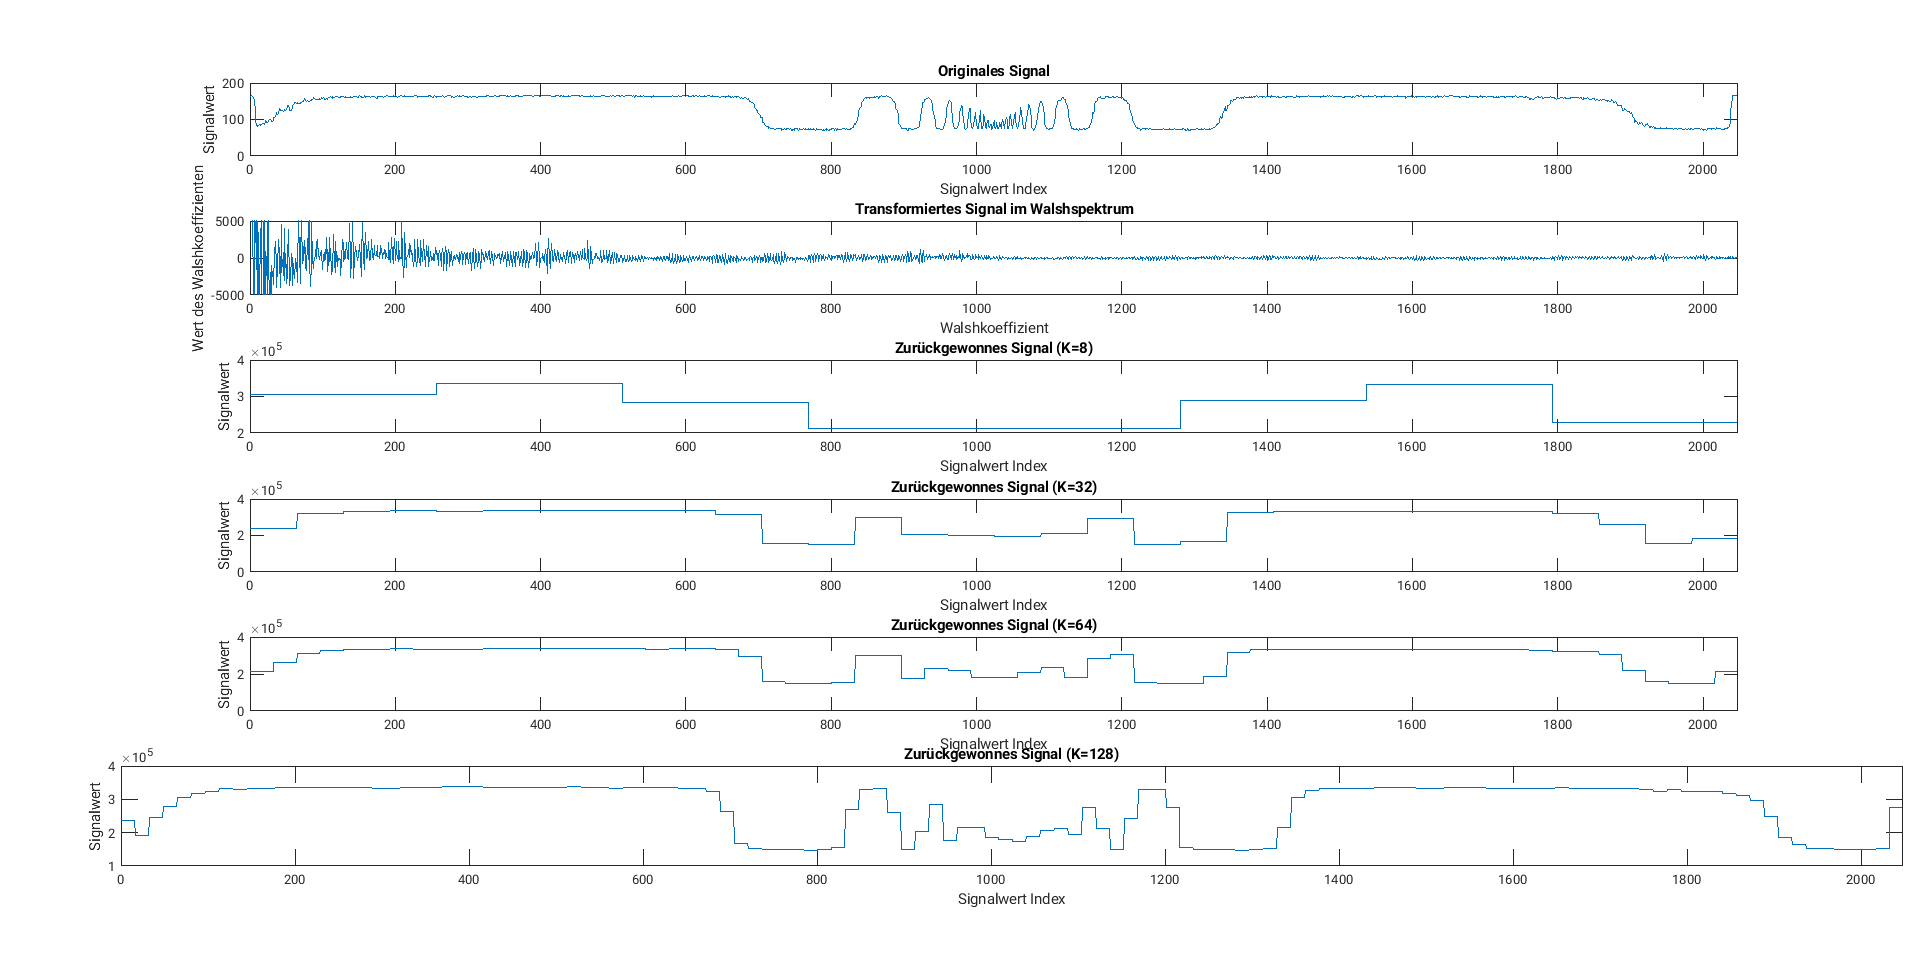
\includegraphics[width = \textwidth]{A40.png}\\
		Dem Spektrum ist zu entnehmen, dass die Walsh-Funktion mit der größten Ähnlichkeiten zum tatsächlichen Signal die Walsh-Funktionen der niedriegen Ordnungen sind. Man kann insbesondere erkennen, dass der Informationsgehalt der ersten 128 Walsh-Koeffizienten so hoch ist, dass durch die Synthese mit nur 128 Koeffizienten ein dem Ausgangssignal grob-ähnliches Signal entsteht. Rudimentäre Eigenschaften sind wiederzuerkennen auch, wenn sich 3 Zehnerpotenzen größer sind.
	
\newpage
	\section*{Übungsaufgabe 42:}
		Nachfolgend ist die Zerlegung der $DWT$ entsprechend der $FFT$ [nach Arbeitsblatt (52)].
		$$
		DFT = \left(\begin{matrix} 1 &0 &0 &0 \\ 0& 0& 1& 0\\ 0& 0& 0& 1 \\ 0& 1& 0& 0\end{matrix}\right) \cdot
		\left(\begin{matrix} 1 &1 &0 &0 \\ 0& 0& 1& 1\\ 1& -1& 0& 0 \\ 0& 0& 1& -1\end{matrix}\right) \cdot
		\left(\begin{matrix} 1 &1 &0 &0 \\ 0& 0& 1& 1\\ 1& -1& 0& 0 \\ 0& 0& 1& -1\end{matrix}\right)
		$$
		Die erste Matrix von links ist eine umsortierte Einheitsmatrix.Folglich wird ihr Beitrag zu dem Gesamtergebnis eine Umordnung des Ergebnisvektors sein.\\
		Die zweite und dritte Matrix entsprechen der Zerlegung der ursprünglichen $DFT$-Matrix modulo einer vorhergehenden Umsortierung der Zeilen. Sie sorgen dafür, dass die Transformation auf eine Addition von benachbarten Vektoreinträgen herunter gebrochen werden kann.\\
		\\
		\begin{tabular}{l | c c c }
			Matrixnummer	&	1.	&	2.	&	3.\\
			\hline
			Nulleinträge	&	12	&	8	&	8\\
			Einseinträge	&	4	&	6	&	6\\
			Andere (-1)		&	0	&	2	&	2\\
			\hline
			Operationen &&&\\
			Addition		&	0	&	4	&	4\\
			Multiplikation	&	0	&	2	&	2\\
			Set-Op			&	3	&	2	&	2\\
		\end{tabular}\\
		\\
		Für ein Signal $s^T = (1,2,3,1)$ und der, wie oben, zerlegten DWT-Matrix $DWT$ gilt folgende Aussage:\\
		\begin{tabular}{r l l}
		$DFT\cdot s =$ &$\left(\begin{matrix} 1 &0 &0 &0 \\ 0& 0& 1& 0\\ 0& 0& 0& 1 \\ 0& 1& 0& 0\end{matrix}\right) \cdot
		\left(\begin{matrix} 1 &1 &0 &0 \\ 0& 0& 1& 1\\ 1& -1& 0& 0 \\ 0& 0& 1& -1\end{matrix}\right) \cdot$&\!\!\!\!\!\!
		$\left(\begin{matrix} 1 &1 &0 &0 \\ 0& 0& 1& 1\\ 1& -1& 0& 0 \\ 0& 0& 1& -1\end{matrix}\right) \cdot
		\left(\begin{matrix} 1\\ 2\\ 3\\ 1 \end{matrix}\right)$\\
		$=$ &$\left(\begin{matrix} 1 &0 &0 &0 \\ 0& 0& 1& 0\\ 0& 0& 0& 1 \\ 0& 1& 0& 0\end{matrix}\right) \cdot
		\left(\begin{matrix} 1 &1 &0 &0 \\ 0& 0& 1& 1\\ 1& -1& 0& 0 \\ 0& 0& 1& -1\end{matrix}\right) \cdot$&\!\!\!\!\!\!
		$\left(\begin{matrix} 3\\ 4\\ -1\\ 2 \end{matrix}\right)$\\
		$=$ &$\left(\begin{matrix} 1 &0 &0 &0 \\ 0& 0& 1& 0\\ 0& 0& 0& 1 \\ 0& 1& 0& 0\end{matrix}\right) \cdot
		\left(\begin{matrix} 7\\ 1\\ -1\\ -3 \end{matrix}\right)$ & \text{(in natürlicher Ordnung)}\\
		$=$ &$\left(\begin{matrix} 7\\ -3\\ 1\\ -1 \end{matrix}\right)$ & \text{(in Squenzordnung)}\\
		\end{tabular}\\
	\\
		Mit dem dazu gehörigen Signalflussgraphen:\\
		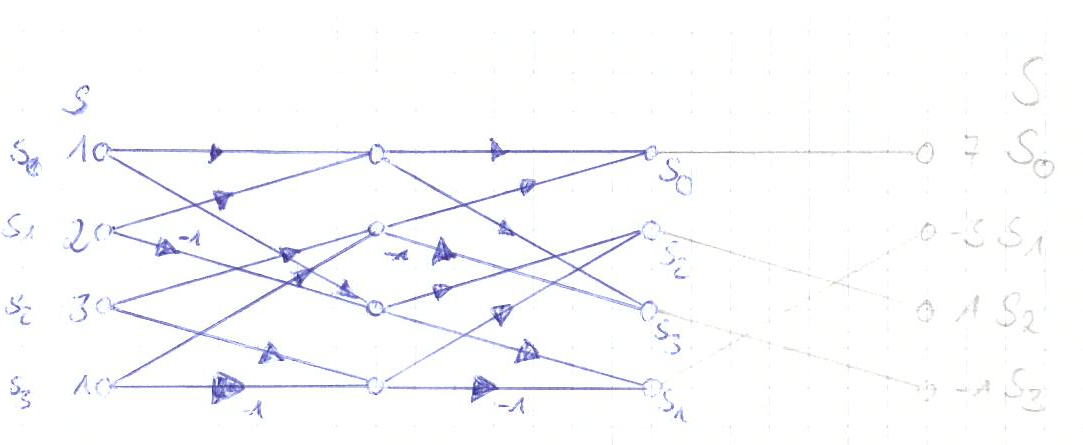
\includegraphics[width = \textwidth]{A42_Signalflussgraph.png}
\newpage\end{document}